\chapter{Physics Object Definitions} \label{chap:objects}

In order to analyze the data one must first reconstruct the detector-level
output into representations of real physical particles (physics objects).  This
process begins once an event is accepted by the ATLAS trigger system and
recorded to disk, as discussed in \Cref{sec:atlas:trigger}.  This raw detector
output, such as energy deposits in the calorimeters or hits in the inner
detector, is then fed into a system of algorithms which build objects of
interest such as jets and muons.  These complex objects can then be used as
representations of the true SM particles in the analysis.  Since these
representations are only as good as the measurement and reconstruction
algorithms, they are then calibrated and given an uncertainty as discussed in
\Cref{chap:systematics}. This chapter gives an overview of the methodology used
to reconstruct the objects required for the boosted $H \rightarrow b\bar{b}$
analysis.

\section{Jets} \label{sec:objects:jets}

The particles that carry QCD color charge do not exist by themselves in
isolation, but instead combine with other colored particles to form colorless
composite hadrons making it impossible to observe individual quarks or gluons
in ATLAS. This process of hadronization, discussed in \Cref{sec:theory:qcd},
creates a shower of charged and neutral particles that leave tracks in the
inner detector and energy deposits in the calorimeters.  Each $pp$ collision
event at the LHC tends to produce a lot of these hadronic showers which are
then clustered into objects known as ``jets."  These jets are intended to
represent the signature of a quark or gluon at leading order.

Jets can be formed from tracks using the hits of charged particles in the ID,
from energy deposits left by both neutral and charged particles in the
calorimeters, or from the truth particles produced via MC.  Since there is
no unique procedure for clustering these signatures, several different
approaches have been developed. The most common clustering options are the
$k_{t}$, Cambridge-Aachen, and anti-$k_{t}$ algorithms \cite{Cacciari:2008gp}.
These algorithms work by iteratively applying the following rules to the
chosen collection of objects:

\begin{enumerate}
  \item Define the distance $d_{iB}$ between the object $i$ and the beamline $B$ in terms of the transverse momentum $\pT$ and $P$ which determines the effect of the energy in the clustering algorithm: \[ d_{iB} = p_{\text{T}i}^{2P} \]
  \item Compute the pairwise distance $d_{ij}$ between objects $i$ and $j$: \[ d_{ij} = \textrm{min}\left(p_{\text{T}i}^{2P}, p_{\text{T}j}^{2P}\right) \frac{\DeltaR_{ij}^{2}}{R^{2}} \] where $\DeltaR_{ij}^{2} = \left(\eta_{i} - \eta_{j}\right)^{2} + \left(\phi_{i} - \phi_{j}\right)^{2}$ is the geometric term dependent on rapidity $\eta$ and the azimuthal angle $\phi$.  $R$ is a parameter which controls the size of the jet.
  \item Choose the smallest distance $d_{\text{min}}$ out of the list of distances: \[ d_{\mathrm{min}} \in \left\{\left\{d_{ij}\right\},\left\{d_{iB}\right\}\right\} \] 
  \item If $d_{\text{min}}$ is the distance between an object, $i$, and the beamline: \[ d_{\mathrm{min}} \in \left\{d_{iB}\right\} \] label this object a jet and remove it from the list
  \item If $d_{\text{min}}$ is the distance between some objects $i$ and $j$: \[ d_{\mathrm{min}} \in \left\{d_{ij}\right\} \] merge objects $i$ and $j$ into a new object $k$, add $k$ to the object collection and remove objects $i$ and $j$.
  \item Repeat until all objects have been clustered into jets and the object collection is empty.
\end{enumerate}

In the above iterative process the choice of parameter P corresponds to three choices of jet clustering algorithm:

\begin{enumerate}

  \item[$P = 1$] This defines the $k_{t}$ algorithm \cite{Catani:1993hr}.  Here the algorithm prioritizes the clustering of soft objects first and then gradually moves on to harder objects.  This has the effect of creating irregular shaped jets that evolve from the ``outside-in" as seen in \Cref{sec:objects:kt}
  \item[$P = 0$] This defines the Cambridge-Aachen algorithm \cite{Dokshitzer:1997in}.  In this case the effect of the energy of the jet is ignored, and instead the jets are clustered based on their geometric distance only.  Again this results in irregular shaped jets as seen in \Cref{sec:objects:Cam_Aachen}
  \item[$P = -1$] This defines the anti-$k_{t}$ algorithm \cite{Cacciari:2008gp}.  This algorithm prioritizes the clustering of hard objects first and then clusters the surrounding softer objects.  This results in mostly cone-like jets which center on the hardest object(s) as seen in \Cref{sec:objects:anti_kt}.
\end{enumerate}

\begin{figure}[!htbp]
  \centering
  \subcaptionbox{$k_{t}$ \label{sec:objects:kt}}{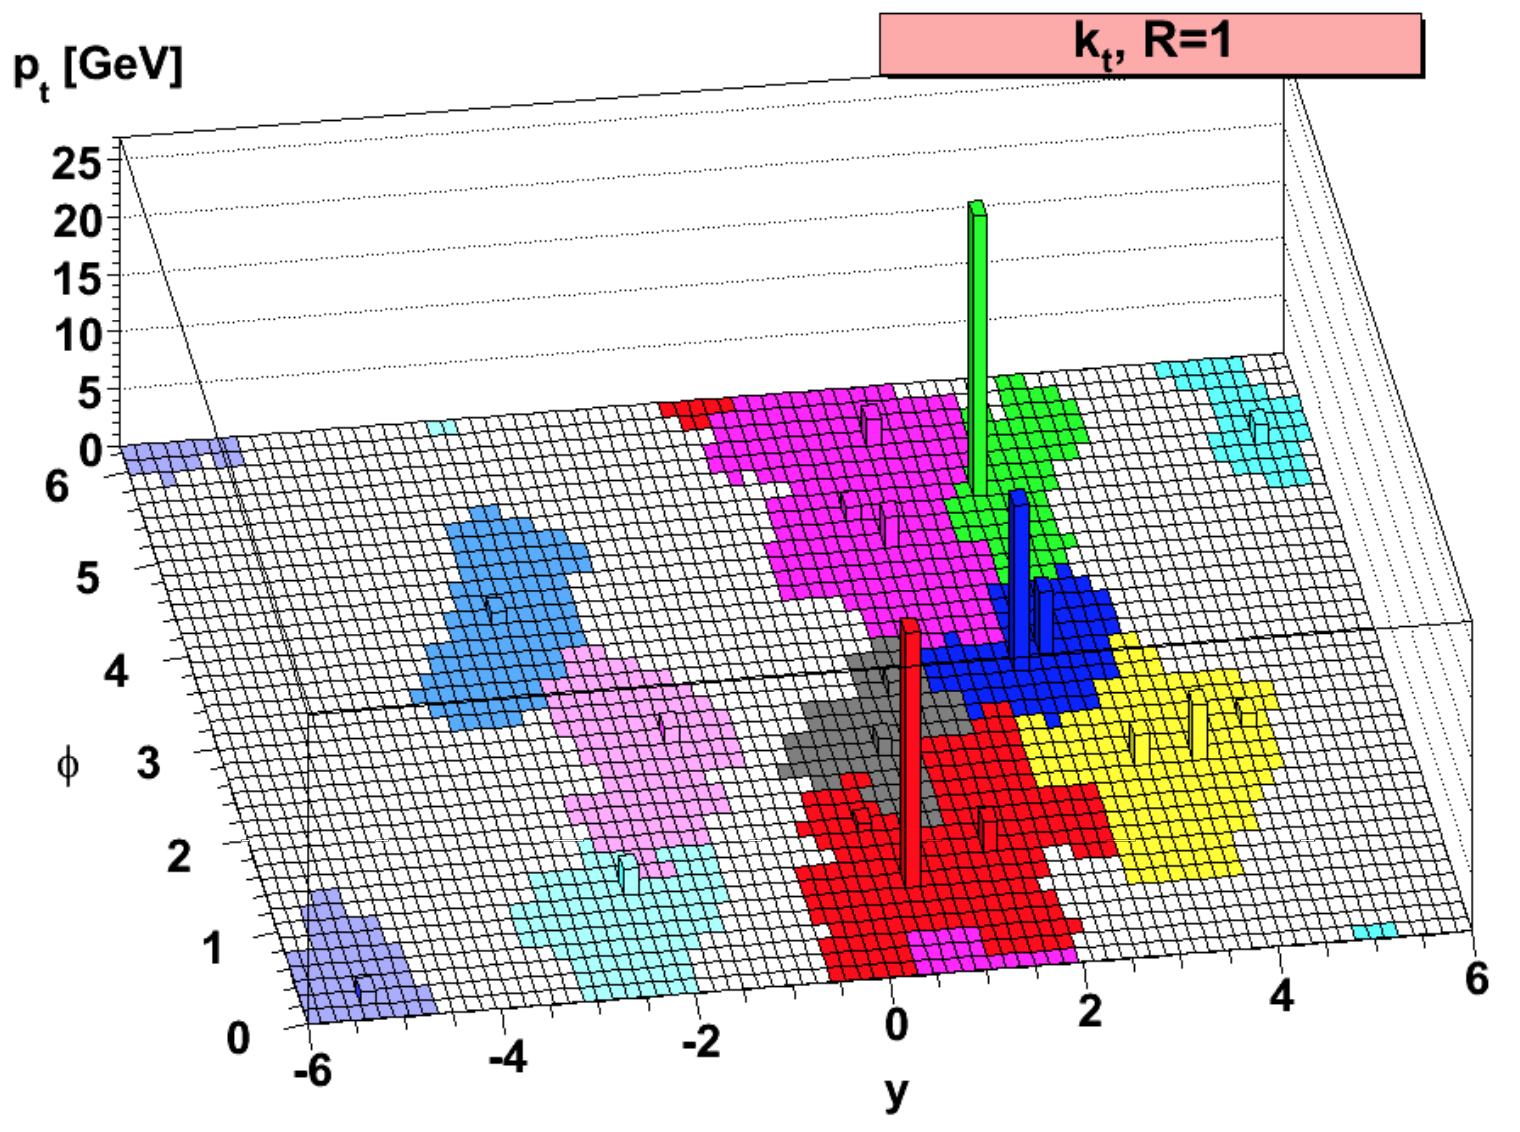
\includegraphics[width=0.32\linewidth]{figures/objects/kt}}
  \subcaptionbox{Cambridge-Aachen \label{sec:objects:Cam_Aachen}}{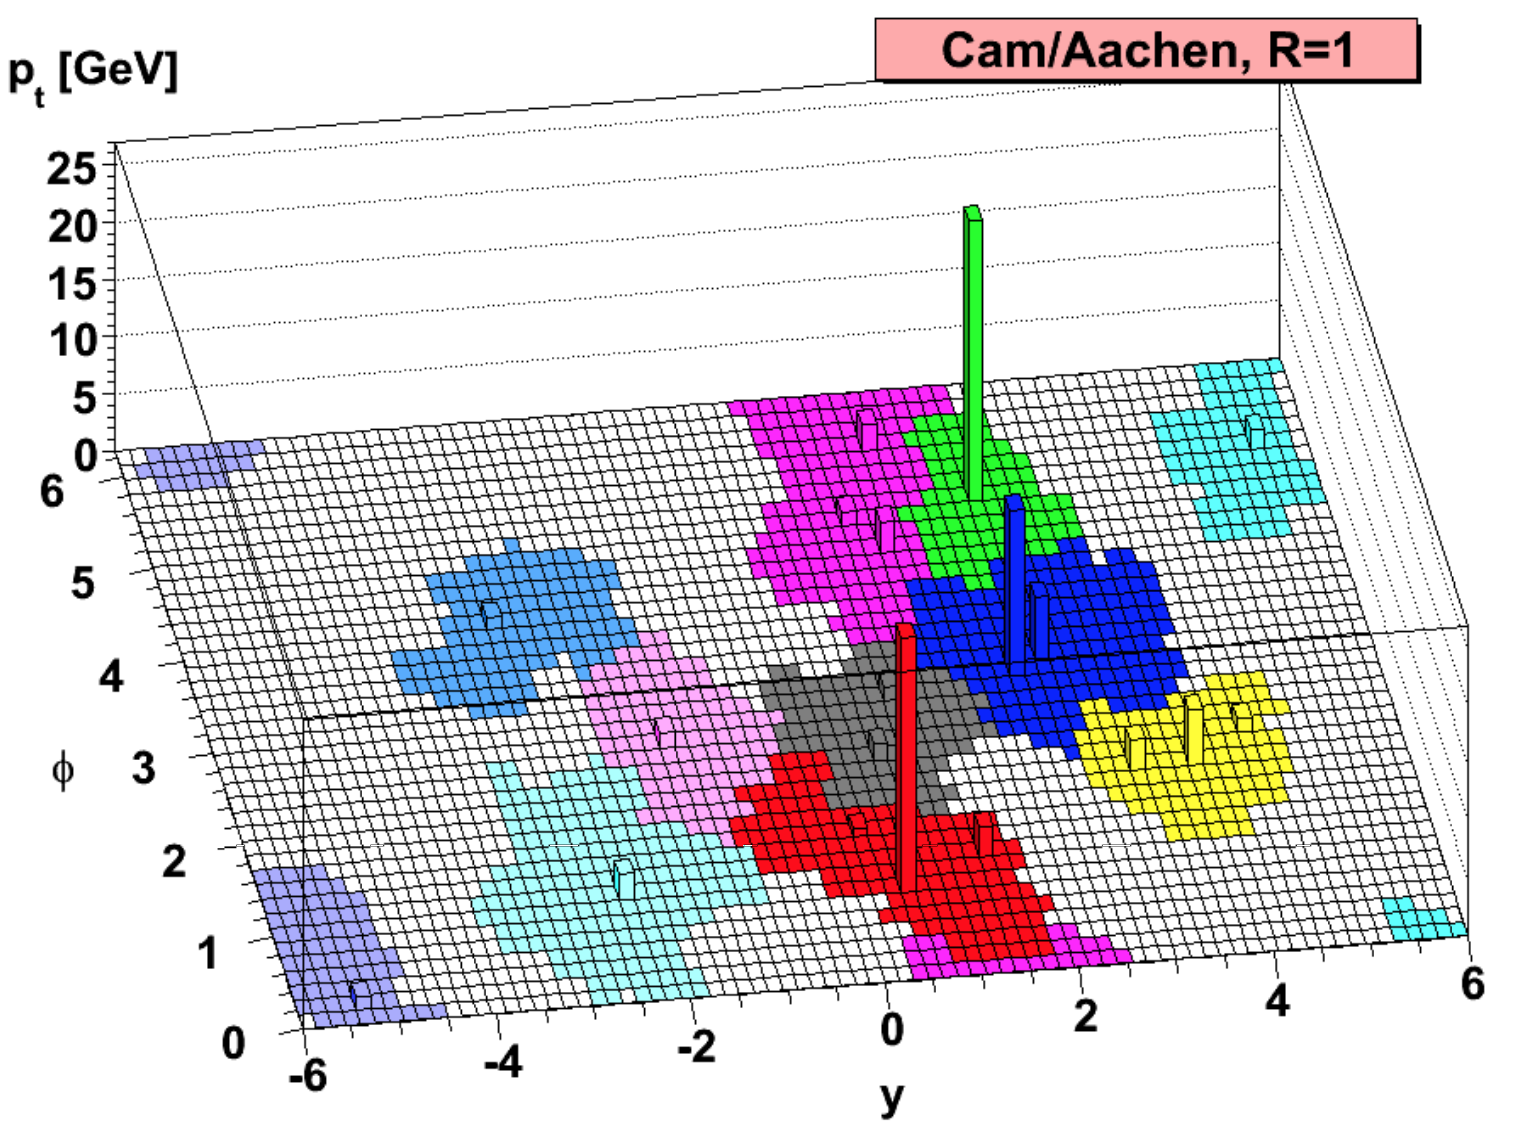
\includegraphics[width=0.32\linewidth]{figures/objects/Cam_Aachen}}
  \subcaptionbox{anti-$k_{t}$ \label{sec:objects:anti_kt}}{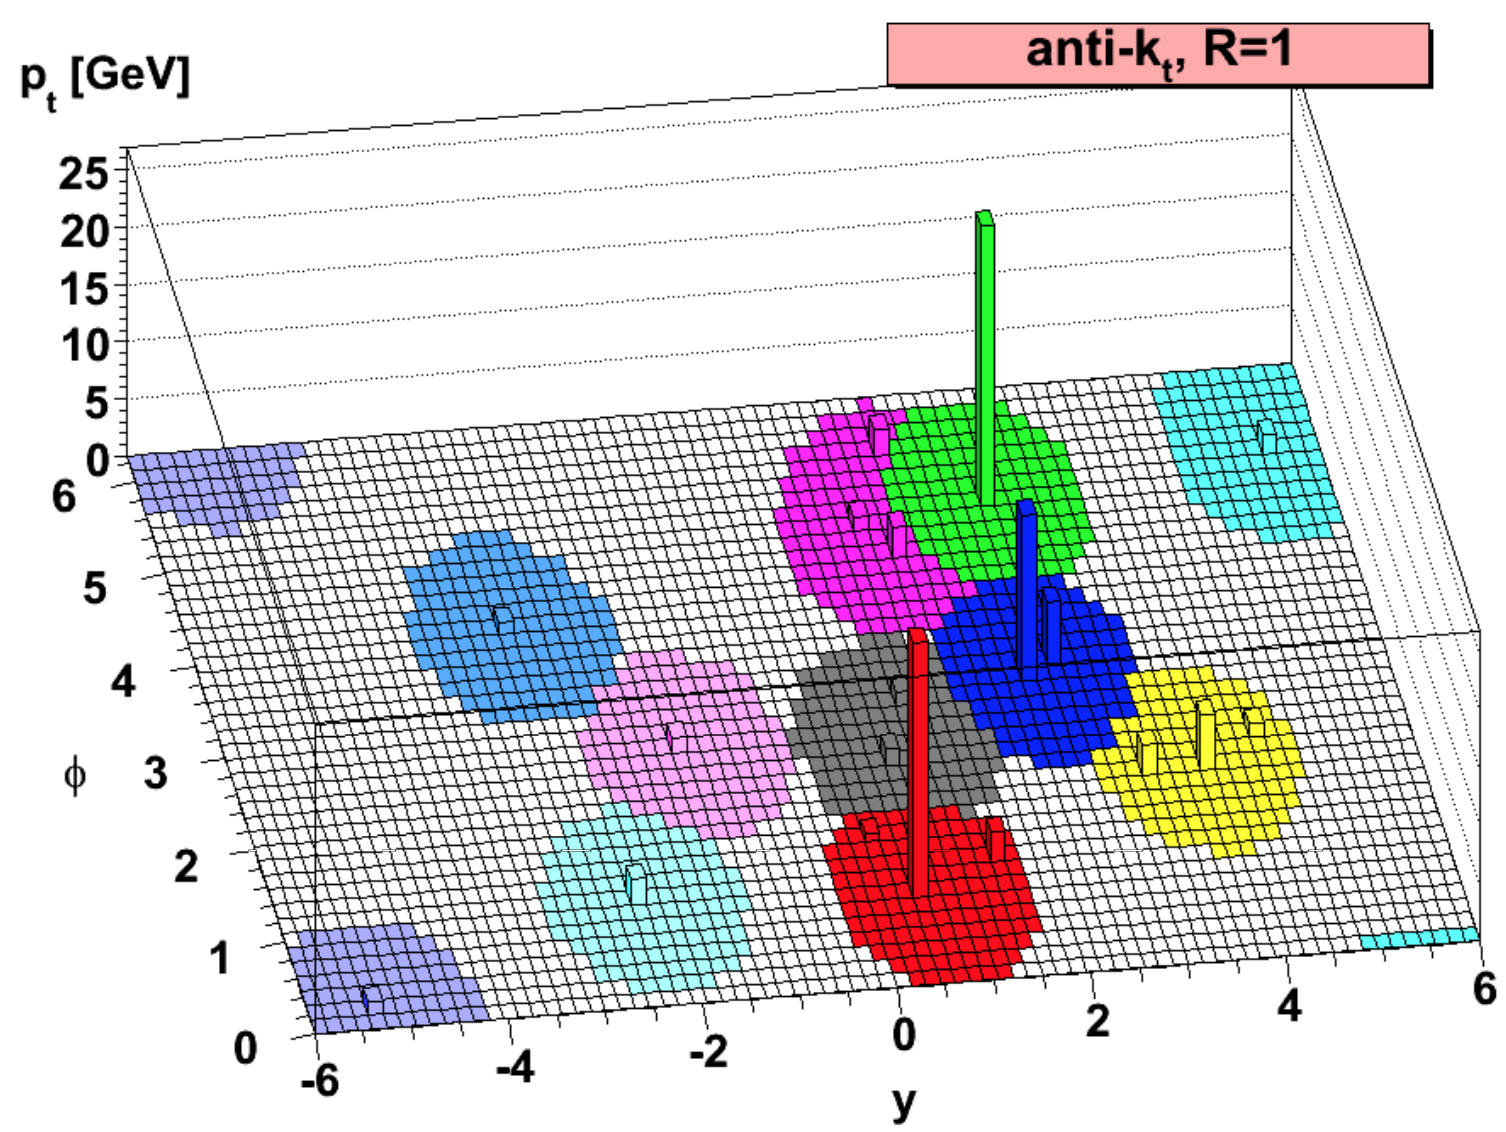
\includegraphics[width=0.32\linewidth]{figures/objects/anti_kt}}
  \caption{Example clustering of a parton-level MC simulation event showing
clustered jet shapes for $R=1.0$ and (a) $P=1$, (b) $P=0$, and (c) $P=-1$
\cite{Cacciari:2008gp}.}
  \label{fig:clustering_algorithms}
\end{figure}

\subsection{Large-$R$ Jets} \label{sec:objects:fatjet}
This dissertation focuses measuring on the boosted signature of the Higgs boson
as it decays to $b\bar{b}$.  As discussed in \Cref{sec:higgs:boosted}, the
resulting decay products are highly collimated and thus can be reconstructed
using a single large radius (``large-$R$") jet.  These large-$R$ jets are
reconstructed from topological calorimeter clusters using the anti-$k_{t}$
algorithm with a radius parameter of $R = 1.0$ resulting in jets similar to
\Cref{sec:object:large_R_example} \cite{Aaboud:2018kfi, Aaboud:2017hdf}. After
clustering the large-$R$ jets are "trimmed" to improve mass resolution and
reduce dependence on pile-up. Trimming is done by first using the $k_{t}$
algorithm to recluster the constituents into subjets with $R=0.2$.  Then any
subjet with $\pT$ less than $5\%$ of the parent large-$R$ jet's energy is
removed \cite{Krohn:2009th}.

\begin{figure}[!htbp]
  \centering
  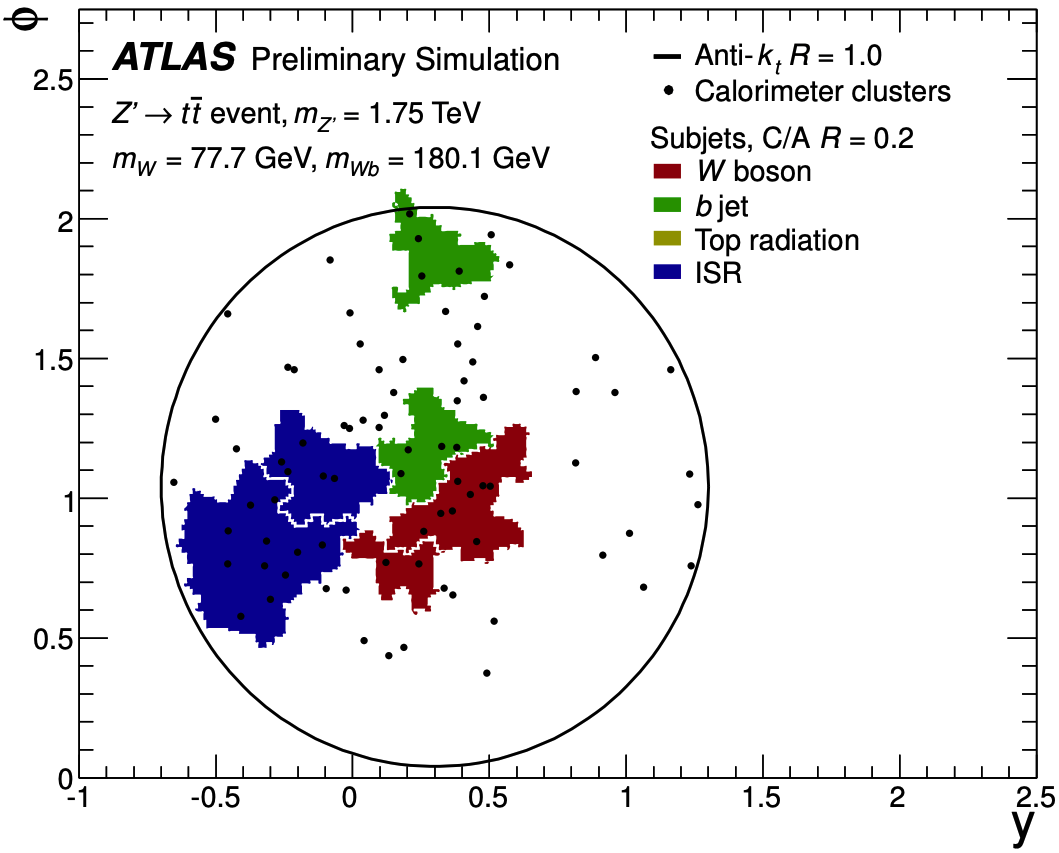
\includegraphics[width=0.7\linewidth]{figures/objects/large_R_example}
  \caption{\cite{ATLAS-CONF-2014-003} Simulation of calorimeter clusters for decay of a boosted $Z' \rightarrow t\bar{t}$ clustered in a large-$R$ jet.}
  \label{sec:object:large_R_example}
\end{figure}

\subsection{Variable Radius Track Jets} \label {sec:objects:vrjets}

After capturing the decay of the Higgs in a large-$R$ jet the next step is to
identify the two sub-jets that represent the $b$ and $\bar{b}$ children of the
Higgs. In this dissertation the Variable Radius (VR) jet was chosen
\cite{Krohn:2009zg,ATL-PHYS-PUB-2017-010} defined by a radius parameter
$R_{\text{eff}}$ which decreases as a function of the jet $\pT$:

\[ R_{\text{eff}}(\pT) = \frac{\rho}{\pT}. \]

The constant $\rho$ determines how quickly the effective size of the VR jet
decreases with respect to the transverse momentum contained inside the jet.  In
this definition the choice of $\rho$ should be proportional to the mass of the
resonance you are attempting to reconstruct and should correctly reproduce the
size of jets as long as $\rho \lesssim 2\pT$. In addition to $\rho$ the VR jet
algorithm requires two additional parameters, $R_{\text{min}}$ and
$R_{\text{max}}$, to impose lower and upper cut-offs on the jet size,
respectively.  These parameters are scanned to optimize the reconstruction of
track jets from $H \rightarrow b\bar{b}$. Using these bounds the
$R_{\text{eff}}$ becomes 

\[
 R_{\text{eff}} \left(\pT\right)= \text{max}\left[\text{min}\left(\frac{\rho}{\pT},R_{\text{max}}\right),R_{\text{min}}\right]\,.
\]

In reconstructing the Higgs boson with $m_{H} = 125~\GeV$, the variable radius
track jet parameters were chosen to be $\rho = 30~\GeV$, $R_{\text{min}}=0.02$,
and $R_{\text{max}}=0.4$, in order to maximize the truth subjet double
$b$-tagging efficiency \cite{ATL-PHYS-PUB-2017-010}, as seen in
\Cref{vr_parameters}.  In \Cref{sec:objects:average_deltaR} the VR Track Jets
properly describe the truth $\Delta R$ distribution for $b$-hadrons while the
$R=0.2$ fixed track jets deviate for higher Higgs jet $\pT$.  Furthermore, in
\Cref{sec:objects:leading_vr} and \Cref{sec:objects:subleading_vr} the VR track
jets do an equally good or better job of identifying the subjets associated
with $b$-hadrons when compared to the $R=0.2$ fixed radius track jets.  This
ability to give a flat efficiency across the entire Higgs $\pT$ spectrum while
accurately describing the topology makes these VR track jets the perfect choice
for this analysis.

\begin{figure}[!htbp]
  \centering
  \subcaptionbox{Study of $\rho$ VR track jet parameter with $R_{\text{min}} = 0.02$ and $R_{\text{max}} = 0.4$}{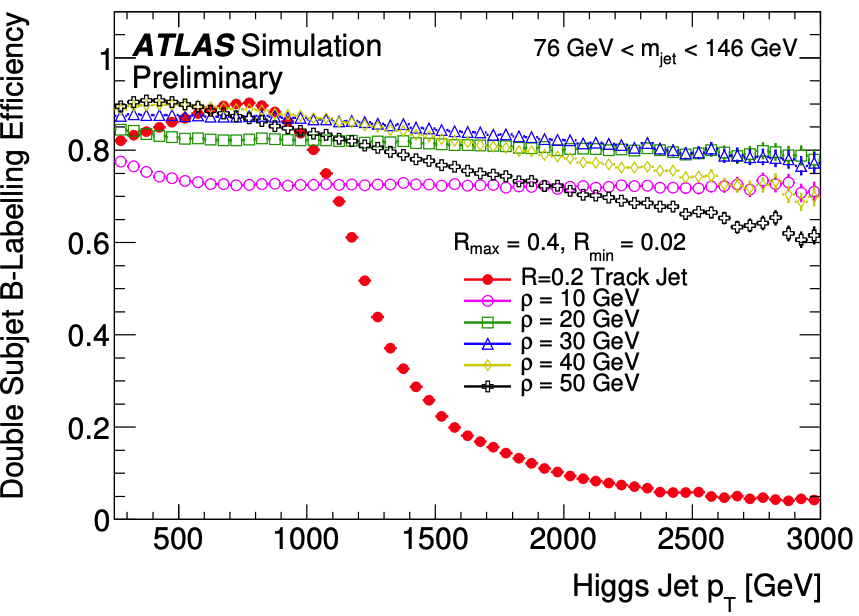
\includegraphics[width=0.48\linewidth]{figures/objects/rho}} \hfill
  \subcaptionbox{Study of $R_{\text{min}}$ VR track jet parameter with $\rho = 30~\GeV$ and $R_{\text{max}} = 0.4$}{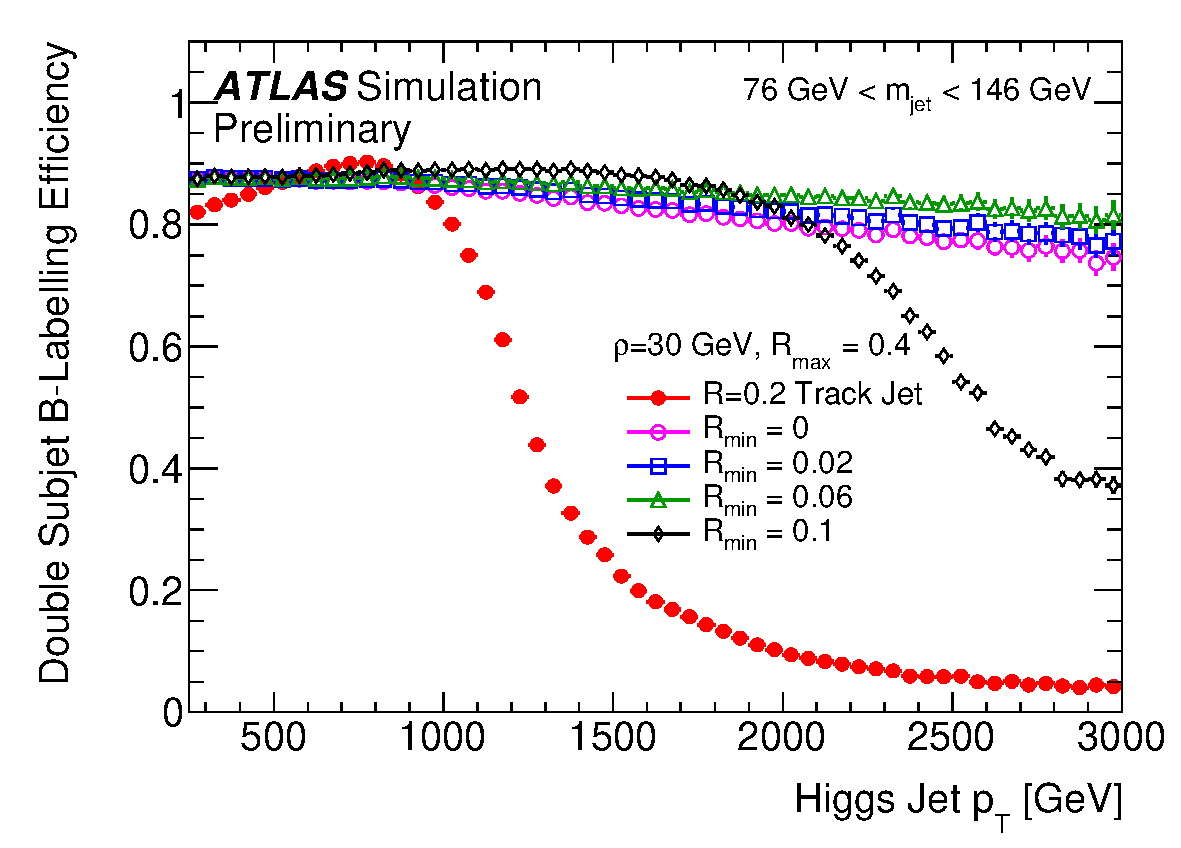
\includegraphics[width=0.48\linewidth]{figures/objects/Rmin}} \hfill
  \subcaptionbox{Study of $R_{\text{max}}$ VR track jet parameter with $\rho = 30~\GeV$ and $R_{\text{min}} = 0.0.02$}{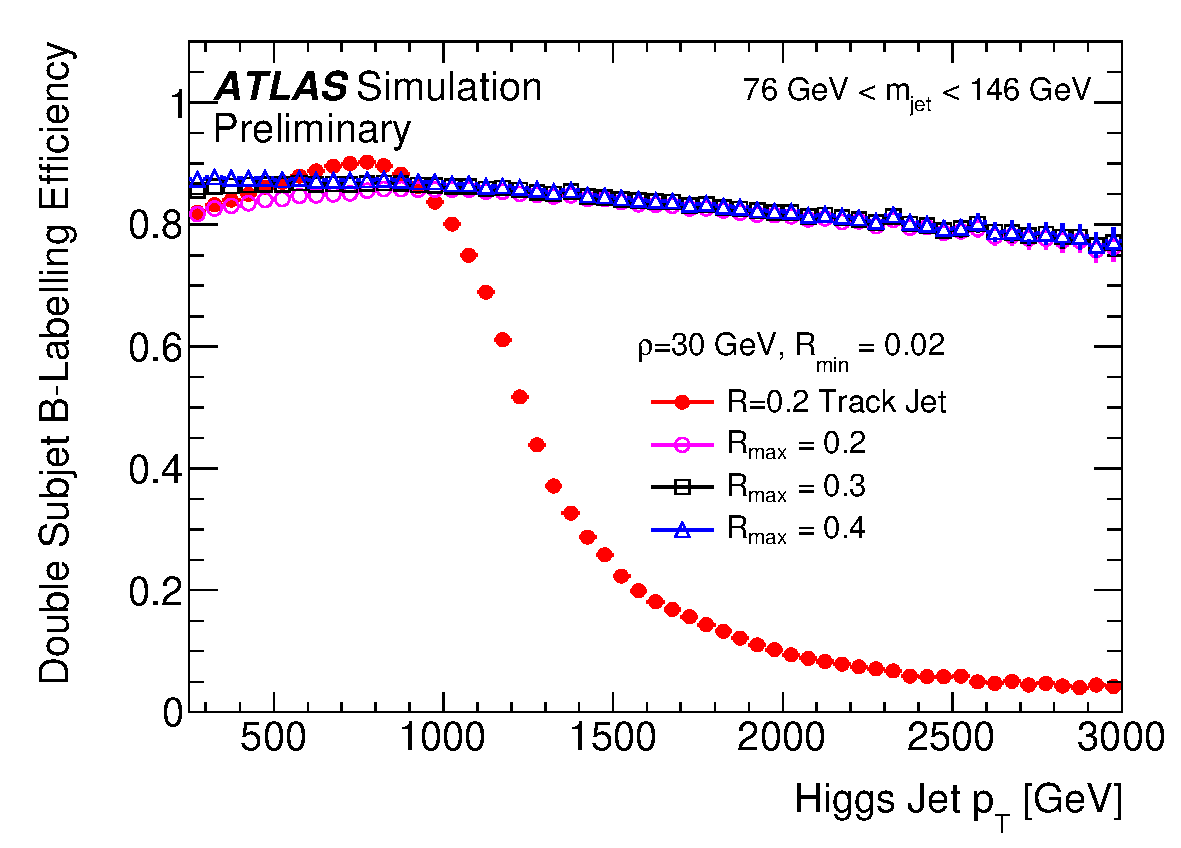
\includegraphics[width=0.48\linewidth]{figures/objects/Rmax}}
  \caption{Labeling efficiency of subjet double $b$-tagging using truth
information from Higgs decay as a function of Higgs jet $\pT$.  The efficiency
for $R=0.2$ fixed radius track jests is included for comparison.  Uncertainty
bars include statistical uncertainties only \cite{ATL-PHYS-PUB-2017-010}.}
  \label{vr_parameters}
\end{figure}

\begin{figure}[!htbp]
  \centering
  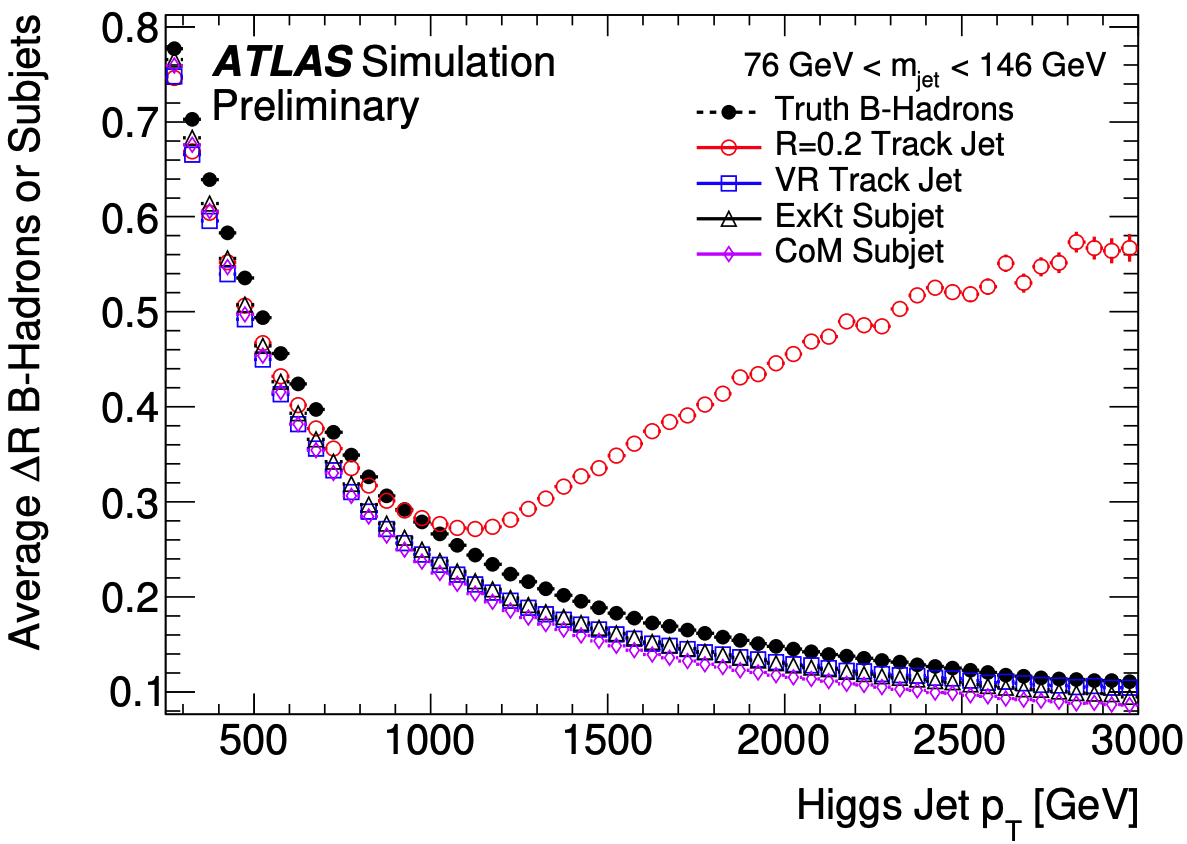
\includegraphics[width=0.98\linewidth]{figures/objects/average_deltaR}

  \caption{\cite{ATL-PHYS-PUB-2017-010} The average $\Delta R$ between either
the two leading truth $b$-hadrons or the two leading subjets associated to a
Higgs jet as a function of Higgs $\pT$}
  \label{sec:objects:average_deltaR}
\end{figure}

\begin{figure}[!htbp]
  \centering
  \subcaptionbox{$250~\GeV$ < Higgs $\pT$ < $400~\GeV$}{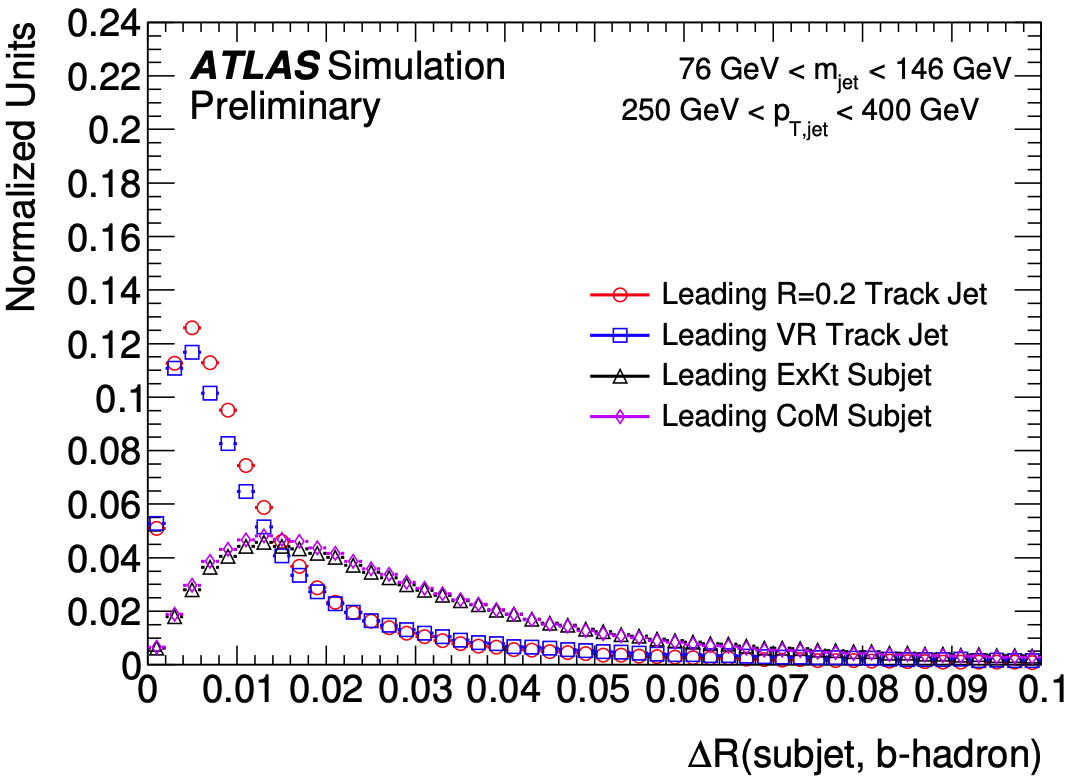
\includegraphics[width=0.48\linewidth]{figures/objects/low_leading_vr}} \hfill
  \subcaptionbox{$800~\GeV$ < Higgs $\pT$ < $1000~\GeV$}{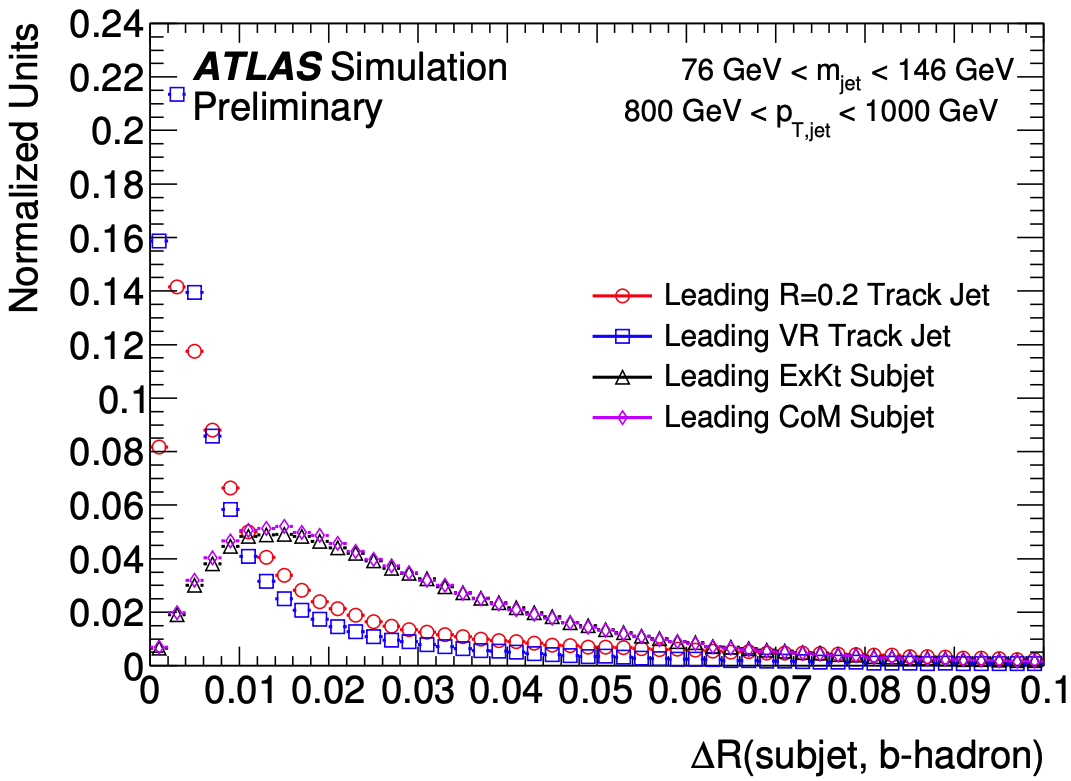
\includegraphics[width=0.48\linewidth]{figures/objects/high_leading_vr}}
  \caption{Distributions of $\Delta R$ between a truth matched $b$-hadron and
the reconstructed leading subjet \cite{ATL-PHYS-PUB-2017-010}.  The
uncertainties given reflect only statistical uncertanties.  All algorithms are
normalized to an area corresponding to the fraction of signal jets which
contain a leading subjet.} 
  \label{sec:objects:leading_vr}
\end{figure}

\begin{figure}[!htbp]
  \centering
  \subcaptionbox{$250~\GeV$ < Higgs $\pT$ < $400~\GeV$}{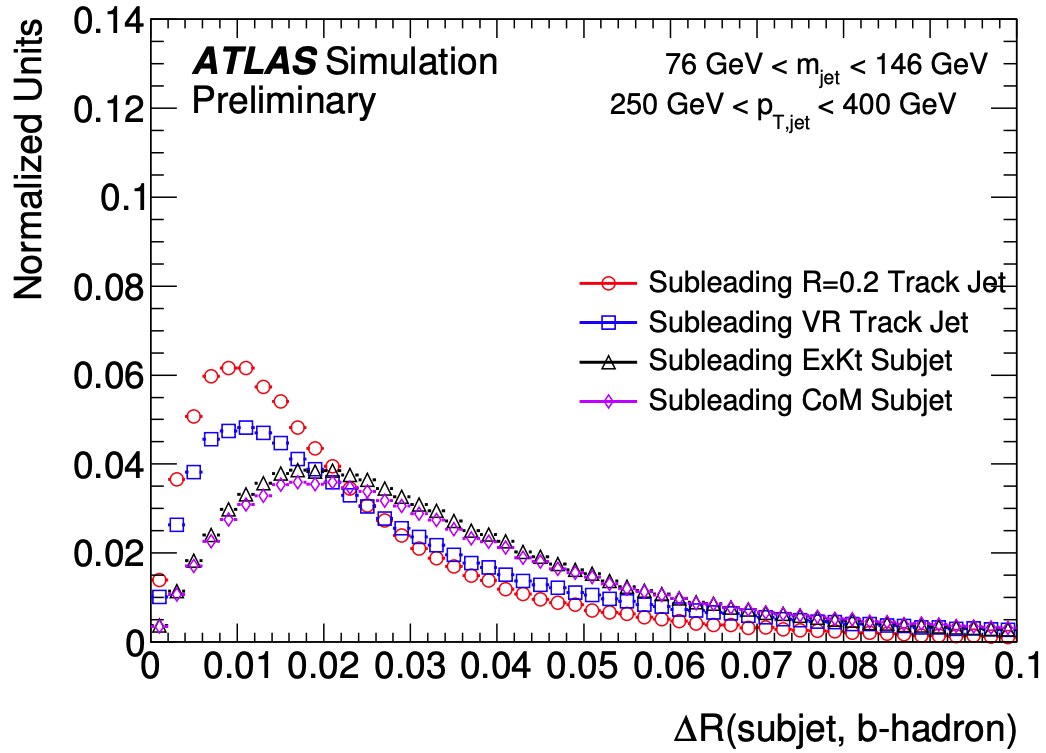
\includegraphics[width=0.48\linewidth]{figures/objects/low_subleading_vr}} \hfill
  \subcaptionbox{$800~\GeV$ < Higgs $\pT$ < $1000~\GeV$}{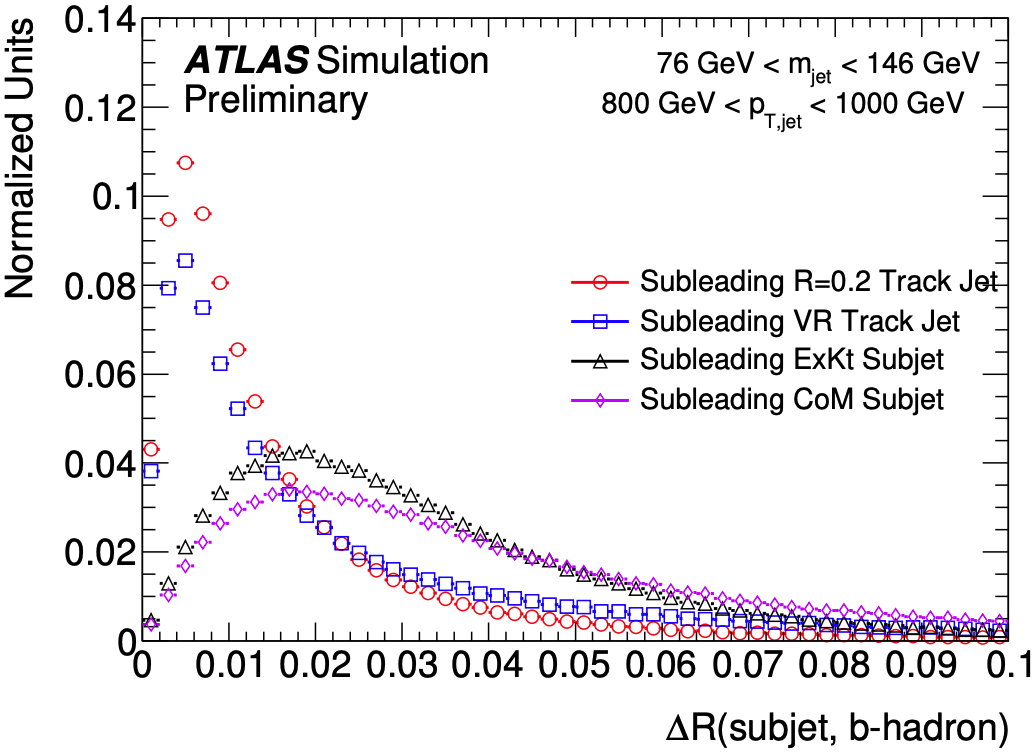
\includegraphics[width=0.48\linewidth]{figures/objects/high_subleading_vr}}

  \caption{Distributions of $\Delta R$ between a truth matched $b$-hadron and
the reconstructed subleading subjet \cite{ATL-PHYS-PUB-2017-010}.  The
uncertainties given reflect only statistical uncertainties.  All algorithms are
normalized to an area corresponding to the fraction of signal jets which
contain a subleading subjet.} 
  \label{sec:objects:subleading_vr}
\end{figure}




\section{Flavor Tagged Jets} \label{sec:objects:flavor_tagging}

In general our reconstruction algorithms for jets are agnostic to the ``flavor"
label - light ($l$), charm ($c$), or bottom ($b$) - of the hadrons produced in
the shower.  However, flavor tagging is a powerful tool for discriminating the
$b\bar{b}$ decay products of the Higgs from the large, predominantly
light-flavor, multijet background \cite{Aad:2015ydr}.  These $b$-quark
initiated jets are identified using the \texttt{MV2c10}
\cite{ATL-PHYS-PUB-2015-022} Boosted Decision Tree (BDT) \footnote{The name
\texttt{MV2c10} means that this multivariate algorithm had a training sample
with roughly $\sim10\%$ $c$-jets and $\sim90\%$ $l$-jets in order to define a
good balance of $c$-jet and $l$-jet rejection.}, trained with a machine learning
algorithm that uses the weighted score from a series of decision trees to give
a discriminant for how similar any given jet is to a $b$-jet.  The BDT uses
inputs from the kinematics of the jet ($\pT$ and $|\eta|$) and the
outputs of tracking algorithms, discussed below, to look for signatures
consistent with a $b$-hadron decay as shown in \Cref{sec:objects:b_decay}.
Tracking information is crucial to flavor tagging, and thus the flavor tagging can only be applied
within the tracking volume ($|\eta| < 2.5$).

\begin{figure}[!htbp]
  \centering
  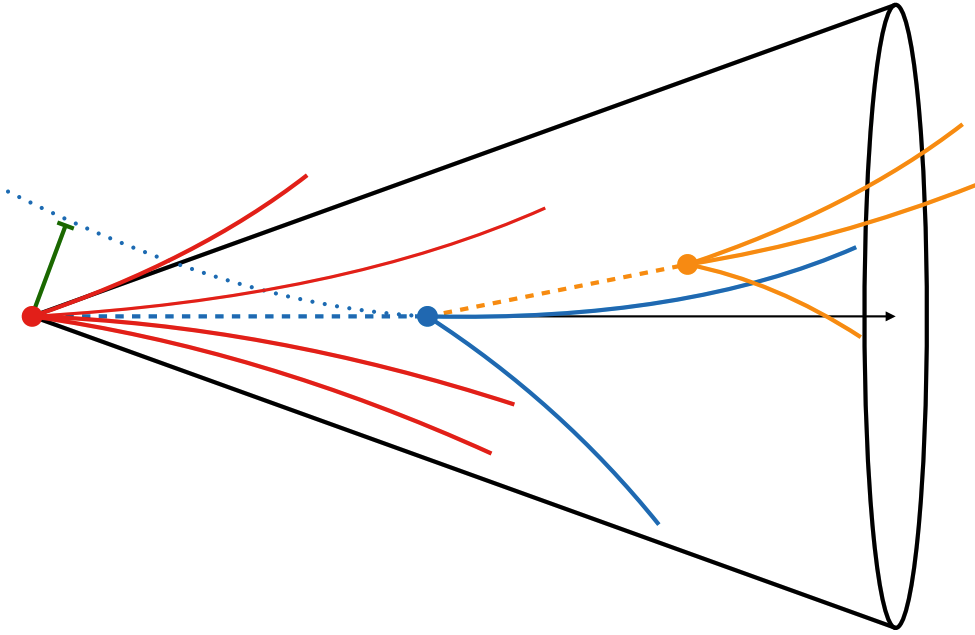
\includegraphics[width=0.8\linewidth]{figures/objects/b_decay}
  \caption{Cartoon of a $b$-jet decay containing a $b$-hadron decay vertex
(\textcolor{track_blue}{blue}~\protect\tikzdot{track_blue}) displaced from the
primary $pp$ vertex (\textcolor{red}{red}~\protect\tikzdot{red}), and a
$c$-hadron decay vertex (\textcolor{orange}{orange}~\protect\tikzdot{orange})
further displaced and often close to the $b$-hadron flight axis
\cite{Chisholm:bjet}. The secondary (\textcolor{track_blue}{blue}) and tertiary
(\textcolor{orange}{orange}) vertices have large impact parameters
(\textcolor{IPgreen}{green}) with respect to the primary $pp$ vertex.}
  \label{sec:objects:b_decay}
\end{figure}

The relatively long lifetime of $b$-hadrons ($\approx 1.5~\ps$) gives them a
characteristic length scale of  $c\tau \sim .45~\mm$. This means the $b$-hadron
travels the non-negligible distance of $\sim 5~\mm$  from the primary
interaction vertex before decaying assuming $\gamma = 10$.  This macroscopic
flight distance is large enough that this decay can be identified as a
secondary vertex (SV) displaced from the original primary vertex (PV).
Furthermore, roughly 90\% of $b$-jets will contain a $c$-jet which will create
a tertiary vertex when it decays (TV) \cite{Chisholm:bjet}.  The secondary
vertex finding algorithm (SV1), and Kalman filter algorithm (JetFitter) look
for events matching this characteristic $b$-hadron decay chain. 

Using tracking information the two-dimensional and three-dimensional impact
parameter algorithms, IP2D and IP3D, determine the transverse and longitudinal
impact-parameters - $d_{\text{0}}$ and $z_{\text{0}}$ - respectively. Looking
at \Cref{sec:objects:impact_parameters} the impact parameters of
the $b$-flavor jets tend to be positive while those of $c$-jets and $l$-jets
tend to be distributed more symmetrically around 0.

\begin{figure}[!htbp]
  \centering
  \subcaptionbox{Transverse Impact Parameter $d_{0}$}{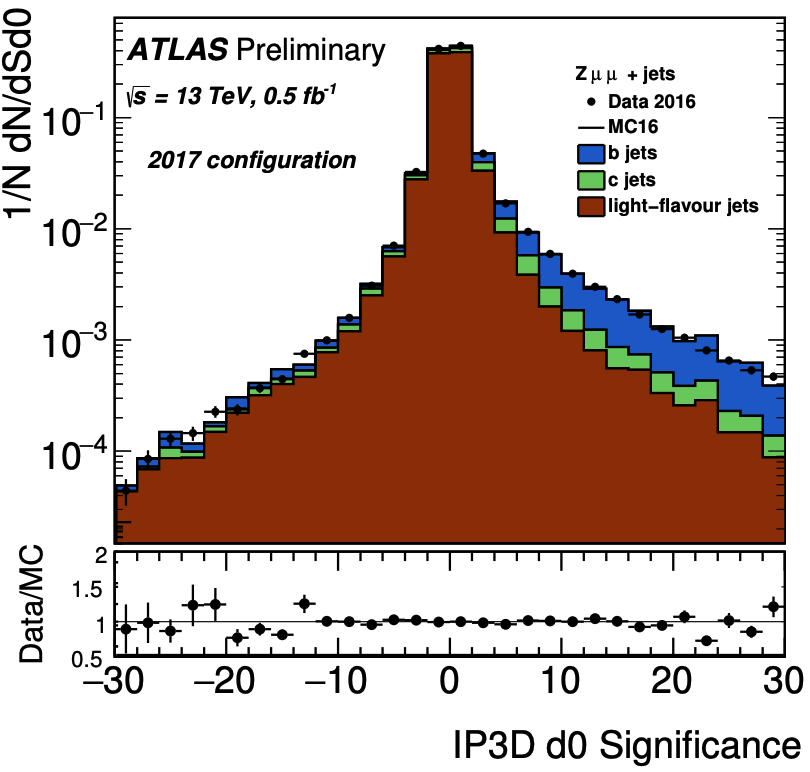
\includegraphics[width=0.48\linewidth]{figures/objects/IP3D_d0}} \hfill
  \subcaptionbox{Longitudinal Impact Parameter $z_{0}$}{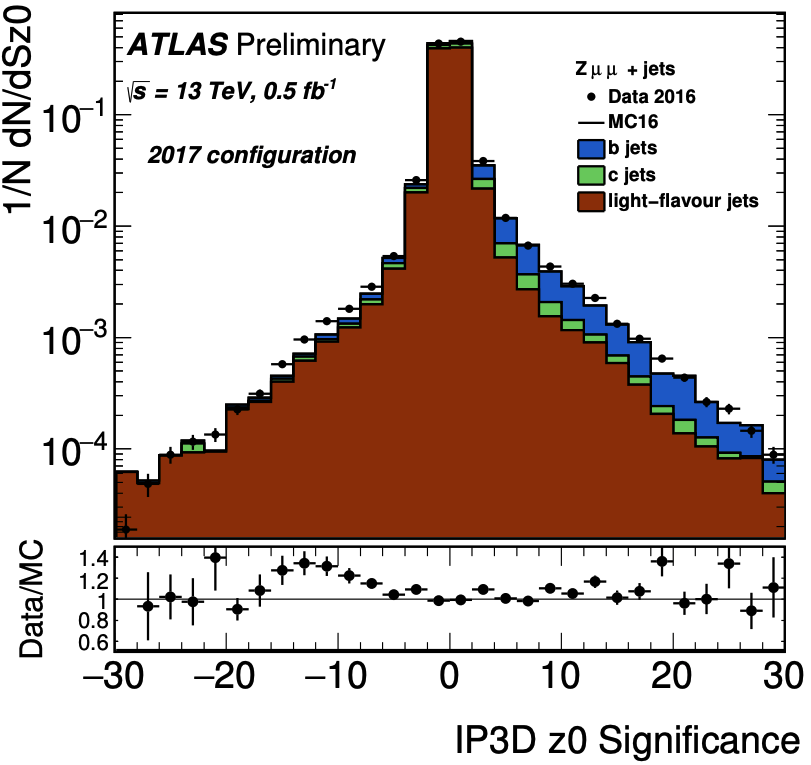
\includegraphics[width=0.48\linewidth]{figures/objects/IP3D_z0}}

  \caption{Data-Monte Carlo comparisons of the
transverse ($d_{0}$) and longitudinal ($z_{0}$) impact parameter significance
values for IP3D selected charged tracks in the leading jet of a $Z\to\mu\mu +
\text{jets}$ dominated sample \cite{Chisholm:bjet}.}
  \label{sec:objects:impact_parameters}
\end{figure}

In 2017 two new tools were included into the tagger
\cite{ATL-PHYS-PUB-2017-013}; a Recurrent Neural Network (RNN) impact parameter
tagger (RNNIP) and a Soft Muon Tagger (SMT).  The RNNIP
\cite{ATL-PHYS-PUB-2017-003} exploits the fact that $b$-jets tend to have many
tracks with highly significant impact parameters, while $l$-jets do not, as
seen in \Cref{sec:objects:RNNIP}.  The SMT \cite{Sciandra:2287545} searches for
muons coming from the semi-leptonic decays of $b$-hadrons and $c$-hadrons to
discriminate against $l$-jets which have much softer muons or none at all. The
separation power of the SMT is shown in \Cref{sec:objects:SMT}.

\begin{figure}[!htbp]
  \centering
  \subcaptionbox{$b$-jets}{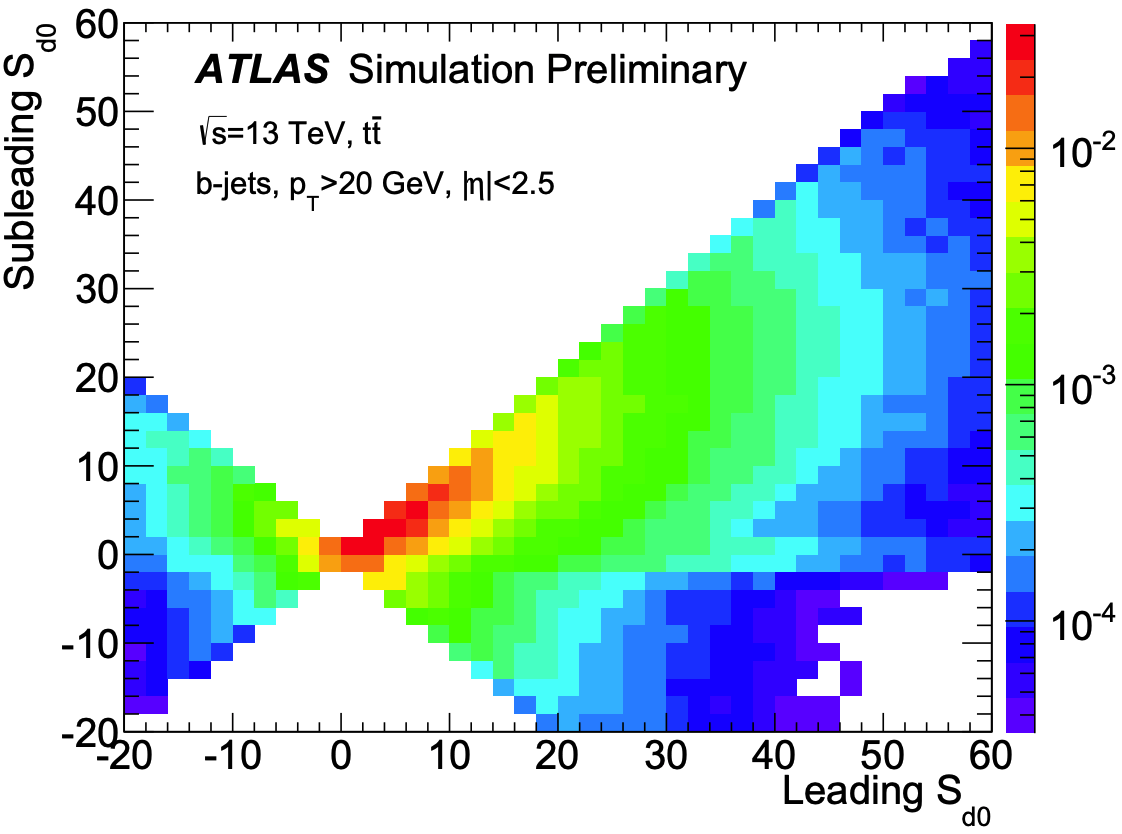
\includegraphics[width=0.48\linewidth]{figures/objects/RNNIP_b_jets}} \hfill
  \subcaptionbox{$l$-jets}{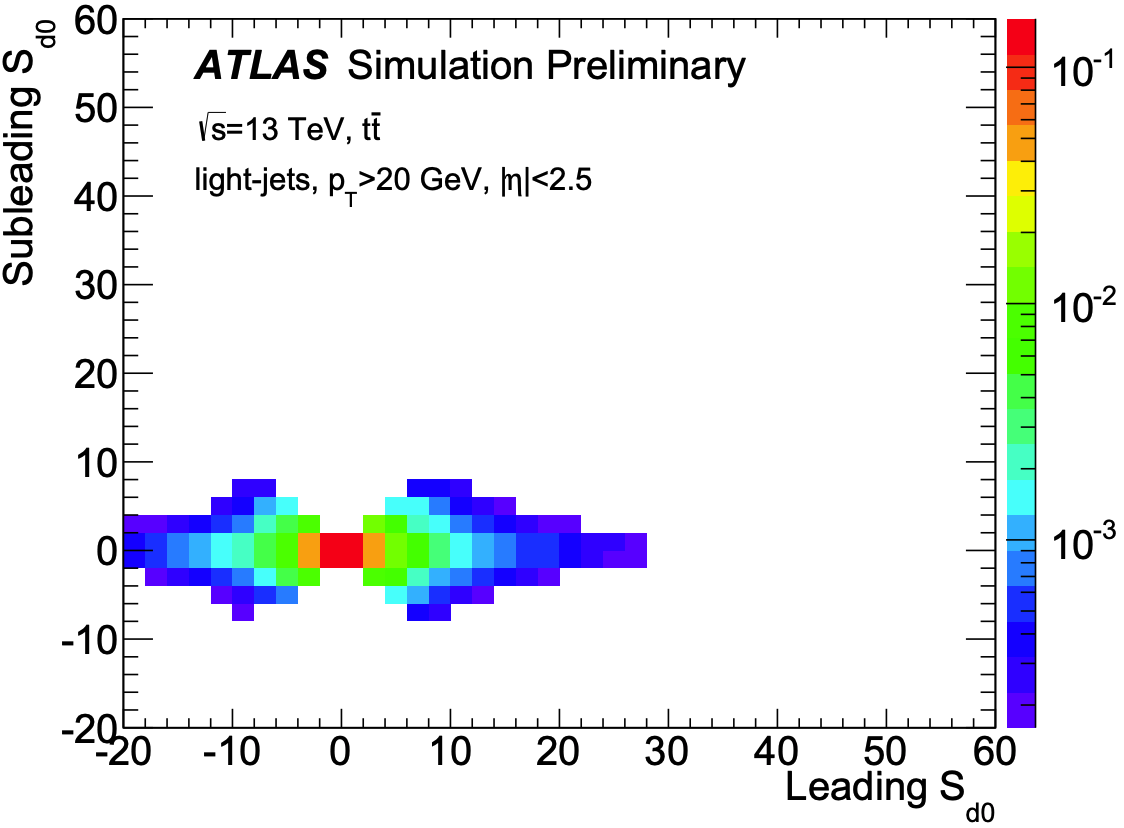
\includegraphics[width=0.48\linewidth]{figures/objects/RNNIP_l_jets}}

  \caption{The distribution of the transverse impact parameter significance $S_{d0}$ for the leading $d_{0}$ significance track and subleading $d_{0}$ significance track for $b$-jets (left) and $l$-jets (right) \cite{Chisholm:bjet}.}
  \label{sec:objects:RNNIP}
\end{figure}

\begin{figure}[!htbp]
  \centering
  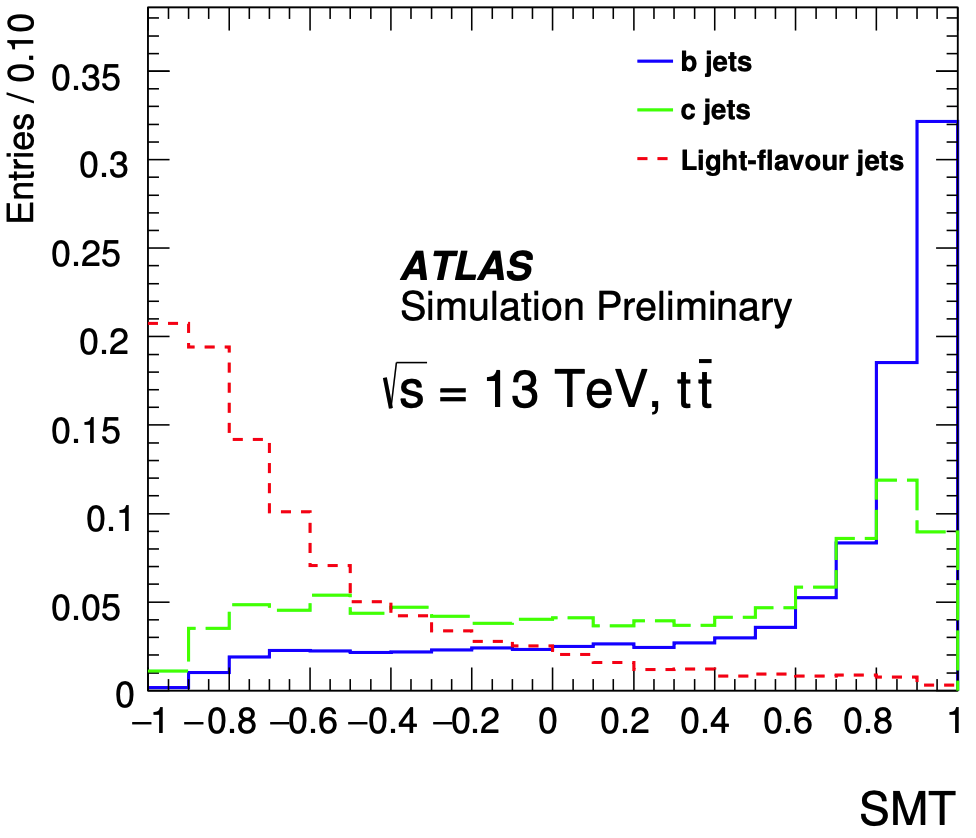
\includegraphics[width=0.5\linewidth]{figures/objects/SMT}
  \caption{Normalized BDT response in simulated $t\bar{t}$ events of the SMT for reconstructed muons associated to $b$-jets (blue), $c$-jets, (green) and light-flavour jets (red) \cite{Chisholm:bjet}.}
  \label{sec:objects:SMT}
\end{figure}

All of the above algorithms' outputs, along with jet kinematic information, are
used as input to the \texttt{MV2c10} algorithm as seen in
\Cref{sec:objects:BDT_flowchart}.  The output is a discriminant score which
indicates how $b$-jet-like or how un-$b$-jet-like the jet in question is,
compared to the training sample used, as shown in
\Cref{sec:objects:MV2c10_output}.  The performance is calibrated in data using
jets containing a muon, indicating the semileptonic decay of the $b$-hadron,
and a correction is derived for the simulated events \cite{Aaboud:2018xwy}.

\begin{figure}[!htbp]
  \centering
  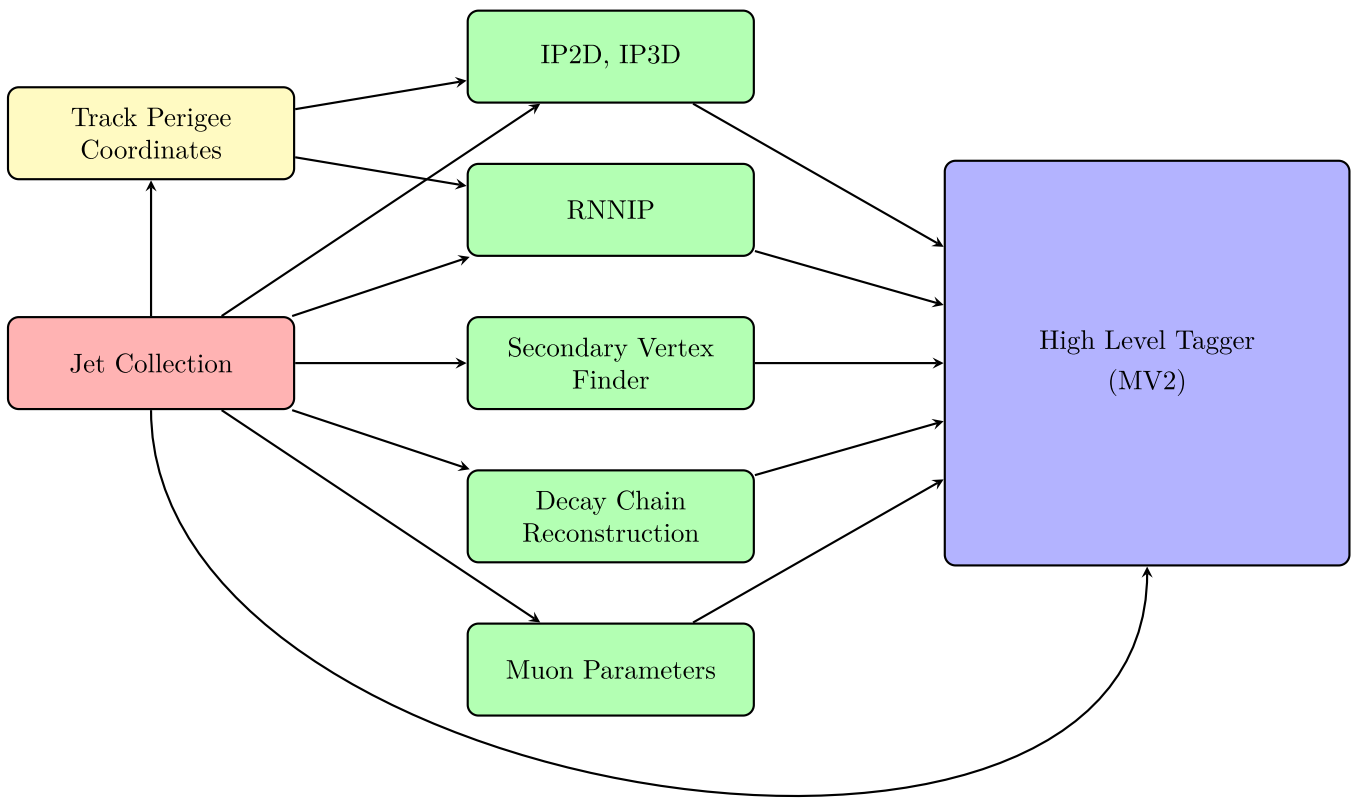
\includegraphics[width=0.8\linewidth]{figures/objects/BDT_flowchart}
  \caption{Flowchart of inputs to the \texttt{MV2c10} $b$-tagging algorithm \cite{Feickert:2690521}.}
  \label{sec:objects:BDT_flowchart}
\end{figure}

\begin{figure}[!htbp]
  \centering
  \subcaptionbox{\texttt{MV2c10} discriminant for $b$-jets compared to $c$-jets and $l$-jets in simulated $t\bar{t}$ events.}{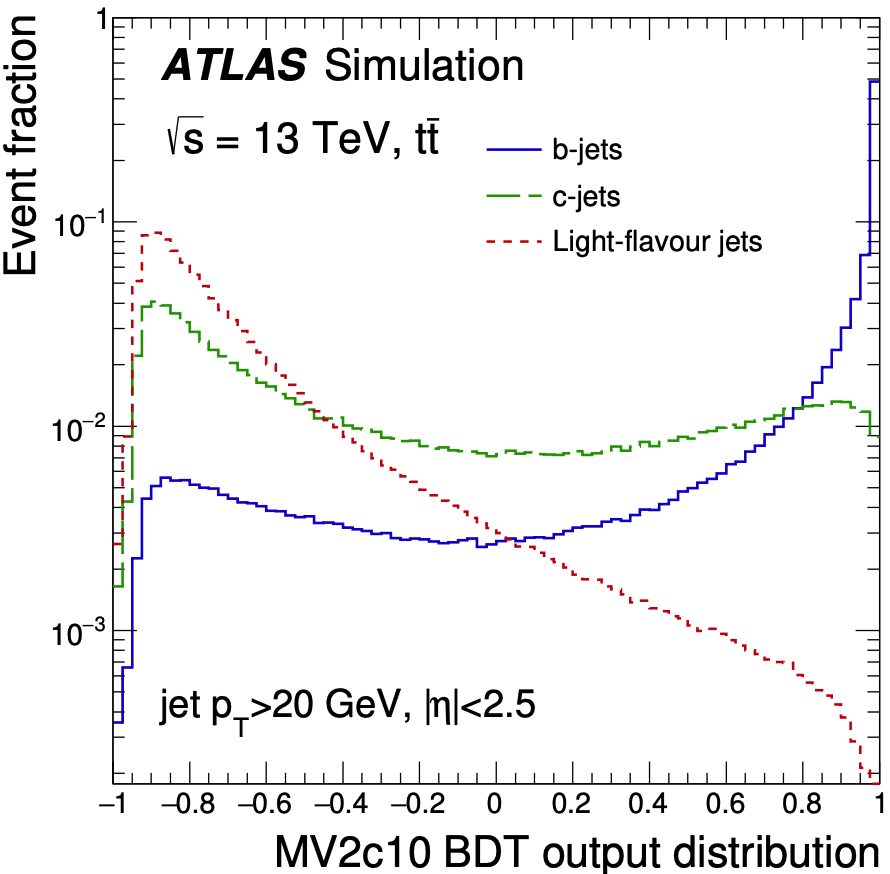
\includegraphics[width=0.48\linewidth]{figures/objects/BDT_output}} \hfill
  \subcaptionbox{$l$-jet and $c$-jet rejection factors as a function of $b$-jet tagging efficiency of the \texttt{MV2c10} BDT.}{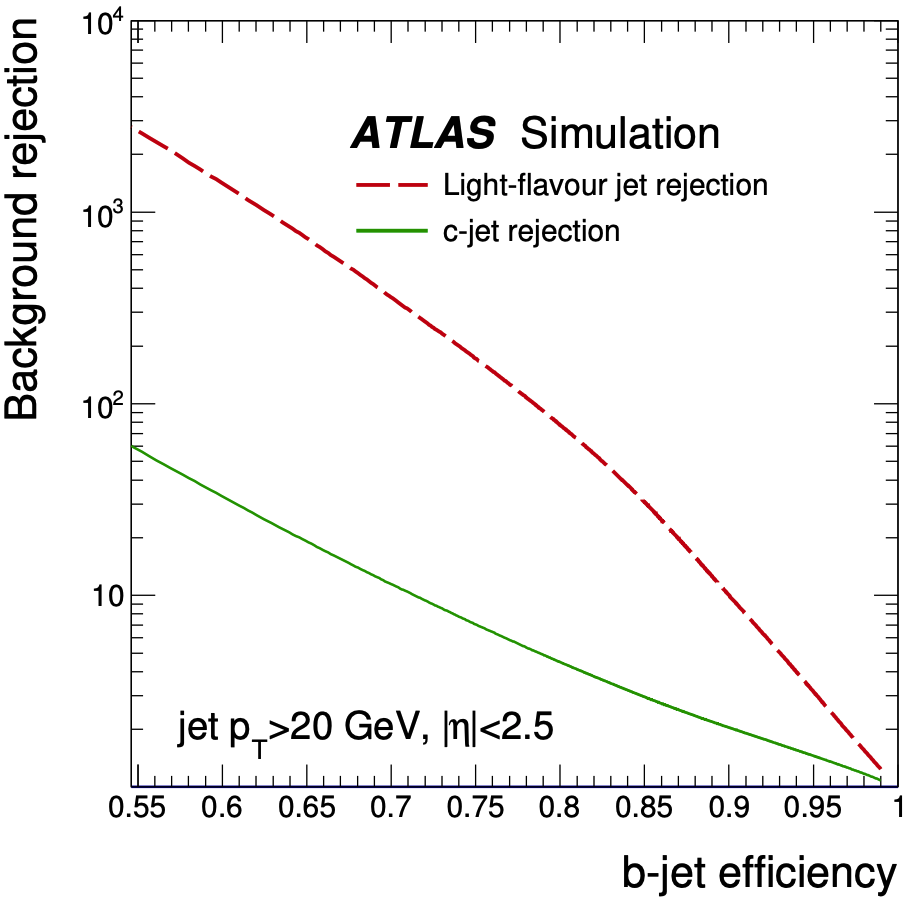
\includegraphics[width=0.48\linewidth]{figures/objects/b_jet_efficiency}}

  \caption{Performance of the \texttt{MV2c10} BDT for
the 2016 optimization in simulated $t\bar{t}$ events.  The performance was
evaluated on $t\bar{t}$ events simulated using \textsc{Powheg} interfaced to
\textsc{Pythia6} \cite{Aaboud:2018xwy}.}
  \label{sec:objects:MV2c10_output}
\end{figure}

\section{Muons} \label{sec:objects:muons}

As muons traverse the entire detector they leave a track of charge deposits in
the Inner Detector (ID) and Muon Spectrometer (MS) which is then reconstructed to
represent the path of the muon \cite{Aad:2016jkr}. This results in four
different muon types, dependant upon which subdetectors were used in the
reconstruction:

\begin{enumerate}
  \item Combined (CB) muons: First the charged track is reconstructed independently in the ID and MS.  Then a global refit combines the hits from both subdetectors. This global fit may add or subtract MS hits from the track to achieve the best fit quality.
  \item Segment-tagged (ST) muons: A track is developed in the ID and then extrapolated to the MS.  If this extrapolation finds at least one local track segment in the MDT or CSC it is labeled a muon.  This is generally used for low $\pT$ muons which may only traverse one layer of the MS.
  \item Calorimeter-tagged (CT) muons: A track formed in the ID is labeled a muon if it can be associated with a calorimeter deposit consistent with a minimum-ionizing particle.  This is the least pure muon type, but it allows for reconstruction of muons that pass through the partially instrumented region of the MS.
  \item Extrapolated (ME) muons: These muons are reconstructed using only MS track information and the loose requirement that the hits are compatible with a trajectory originating from the interaction point.  This type is useful for extending the muon acceptance into the region not covered by the ID.
\end{enumerate}

After the muon type is determined the quality of the muon is categorized by
requiring a specific number of hits in each subcomponent.  These quality
requirements are provided to address the specific needs of different physics
analysis. The four muon quality levels are defined:

\begin{enumerate}
  \item[\texttt{loose}] The lowest quality is designed to maximize the reconstruction efficiency for muons by allowing all muon types to be used.  This is primarily useful for analyses of multi-leptonic final states such as $H \rightarrow 4\ell$.
  \item[\texttt{medium}] The medium quality is designed to minimize the systematic uncertainties associated with muon reconstruction and calibration.  Only CB and ME tracks are used, with at least 3 CB track hits and at least 3 ME layers.  This is the default quality selection in ATLAS and the one used for muons in this analysis.
  \item[\texttt{tight}] This selection maximizes the purity of muons but reduces the reconstruction efficiency. Only CB muons with at least 2 layers of the MS that also satisfy the \texttt{medium} selection requirements are allowed.
  \item[\texttt{high-$\pT$}] Designed to optimize the momentum resolution for tracks with $\pT > 100~\GeV$.  This selection only includes CB muons with hits in at least two layers of the MS that also satisfy the \texttt{medium} selection requirements. This quality level is mostly used for high-mass $W'$ and $Z'$ analyses.
\end{enumerate}

The final step for muon reconstruction is to check that the muon is well
isolated, in order to suppress muons resulting from meson and heavy-flavor decays. This
is done using both the track-based ($\pT^{\text{varcone}30}$) and the
calorimeter-based ($E_{\text{T}}^{\text{topocone}20}$) isolation-based variables which
represent the scalar sum of $\pT$ inside a $\Delta R < 0.3$ cone and the
scalar sum of $E_{\text{T}}$ inside a $\Delta R < 0.2$ cone.  Taking the ratio of
these variables to the total $\pT$ of the candidate muon gives a sense of
how much radiation is surrounding the core of the muon in question. Many
different isolation working points are established by cutting on these ratio
distributions. For this analysis the \texttt{loose} working point was chosen which gives a
$99\%$ muon reconstruction efficiency constant in $\eta$ and $\pT$ as
measured in both a simulated $Z \rightarrow \mu\mu$ sample and data \cite{Aad:2016jkr}.

After reconstruction, these muons are calibrated to data using the well understood
decay $J/\Psi \rightarrow \mu^{+}\mu^{-}$ to cover the low $\pT$ spectrum and
$Z \rightarrow \mu^{+}\mu^{-}$ for the high $\pT$ spectrum, as shown in \Cref{sec:objects:medium_muons}.

\begin{figure}[!htbp]
  \centering
  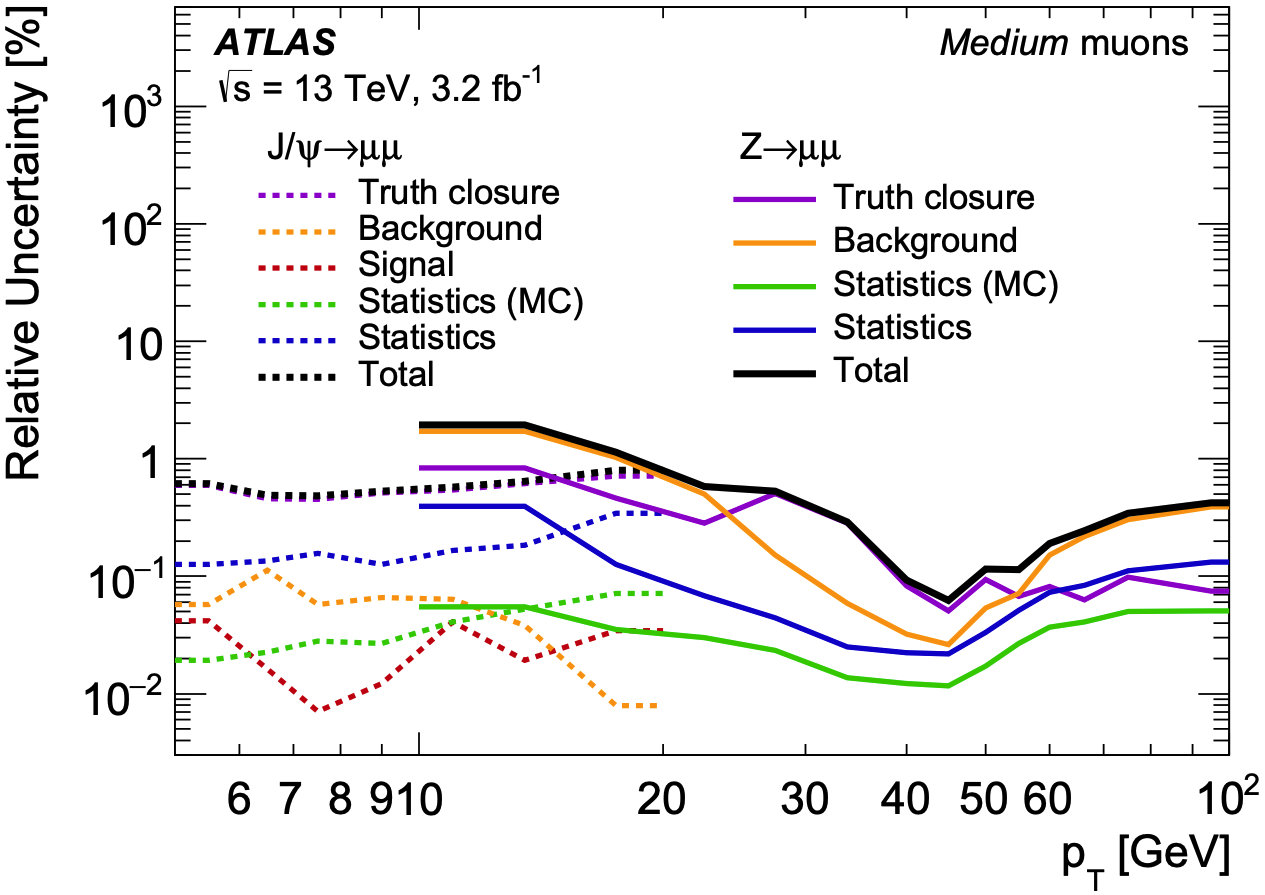
\includegraphics[width=0.8\linewidth]{figures/objects/medium_muons}
  \caption{Total uncertainty in the efficiency scale factor for Medium muons as a function of $\pT$ as measured in $Z \rightarrow \mu\mu$ (solid lines) and $J/\Psi \rightarrow \mu\mu$ (dashed lines) decays. The combined uncertainty is the sum in quadrature of the individual contributions \cite{Aad:2016jkr}.}
  \label{sec:objects:medium_muons}
\end{figure}

